\chapter{Experimental Setup}
\label{chap:setup}

This chapter documents the hardware apparatus, data-collection protocol, and software pipeline used to evaluate the causal, per-event cancellation method described in Chapters~\ref{chap:problem}--\ref{chap:cancellation}. Our goal is to provide enough detail for faithful reproduction: sensor and rig configuration, calibration steps, sequence design, and the end-to-end processing stack (estimation $\rightarrow$ prediction $\rightarrow$ gating $\rightarrow$ metrics).

% ============================================================
\section{Hardware and Apparatus}
\label{sec:hardware}

\subsection{Event Camera and Optics}
We used a single event-based sensor mounted on a rigid aluminum frame facing a rotating disc (Fig.~\ref{fig:rig}). The relevant characteristics:

\begin{itemize}
  \item \textbf{Sensor:} Prophesee Gen4 event camera (1280$\times$720). Timestamp precision on the order of microseconds; polarity encoding in $\{\pm1\}$ (or $\{0,1\}$). Dynamic range $\sim$120\,dB \cite{Finateu2020ISSCC}.
  \item \textbf{Lens:} Standard C-mount lens, focal length selected to provide adequate field of view for the disc. Focus was carefully set at the disc plane to maximize edge sharpness and contrast. Aperture chosen to avoid saturation while maintaining high contrast on the textured disc patterns.
  \item \textbf{Mounting:} Camera mounted on a tripod aimed at the rotating disc. The optical axis was approximately orthogonal to the disc plane over the region of interest.
  \item \textbf{Working distance:} Approximately 60--80\,cm from sensor to disc plane (calibrated via known disc diameter and imaged radius), yielding an imaged disc radius of 264\,px at the chosen focal length. This provided sufficient spatial resolution for motion estimation and cancellation analysis.
\end{itemize}

\subsection{Spinning Disc Rig}
The target is a flat wooden disc with an \emph{uneven, high-contrast pattern} adhered to the visible face to generate rich edge structures under rotation (Fig.~\ref{fig:rig}). Hardware elements:

\begin{itemize}
  \item \textbf{Disc:} Circular wooden plate approximately 30--40\,cm in diameter, with thickness sufficient to maintain rigidity under rotation. Six square paper patterns are affixed to the disc face using blue tape at the corners, creating a grid layout (visible in Fig.~\ref{fig:rig}). The patterns consist of:
  \begin{itemize}
    \item Four squares with intricate, flowing concentric black and white lines resembling topographical contours or fingerprint patterns, providing dense, curved edge structures.
    \item Two squares (top corners) with dense random assortments of black and white shapes including squiggles, hearts, stars, circles, and crosses, creating high-frequency spatial content.
  \end{itemize}
  These patterns generate a rich variety of edge orientations and spatial frequencies to stress-test the cancellation algorithm across different geometric configurations.
  \item \textbf{Actuation:} Precision DC or BLDC motor with controller; rotation rate adjustable via voltage or PWM command from the test equipment (visible on top shelf in Fig.~\ref{fig:rig}). Nominal speeds tested: 1.5--3.5\,rev/s, corresponding to angular velocities $\omega \approx 1.5--3.5$\,rad/s, with steady-state angular velocity ripple below 2\% after warm-up.
  \item \textbf{Spindle and bearings:} Low-runout precision bearings support the spindle to minimize lateral wobble and eccentricity. A hub mount ensures concentricity between the disc and rotation axis, maintaining stable circular motion for consistent experimental conditions.
  \item \textbf{Coordinate system:} A red hand-drawn coordinate system on the grey mounting board (visible in Fig.~\ref{fig:rig}, lower-left) defines the reference frame with $x$ pointing right and $y$ pointing down, consistent with image-plane conventions.
\end{itemize}

\subsection{Lighting Conditions}
Event generation depends on brightness gradients and texture. We used ambient room lighting only (curtains closed to minimize external variation); no external lighting was employed. Illumination varied slightly with the room lights but was stable during each sequence.

\subsection{Calibration and Referencing}
We performed lightweight calibration sufficient for short-horizon rotation modeling:

\begin{itemize}
  \item \textbf{Intrinsics/distortion:} No intrinsic calibration was performed. Processing was done in pixel coordinates; distortion was not explicitly compensated.
  \item \textbf{Disc center in image:} Estimated via circle fitting on short event windows; see Chapter~\ref{chap:motion} for the method.
  \item \textbf{Angular velocity reference:} Estimated by angle differencing around the fitted center with causal smoothing; see Chapter~\ref{chap:motion}.
\end{itemize}

\begin{figure}[t]
  \centering
  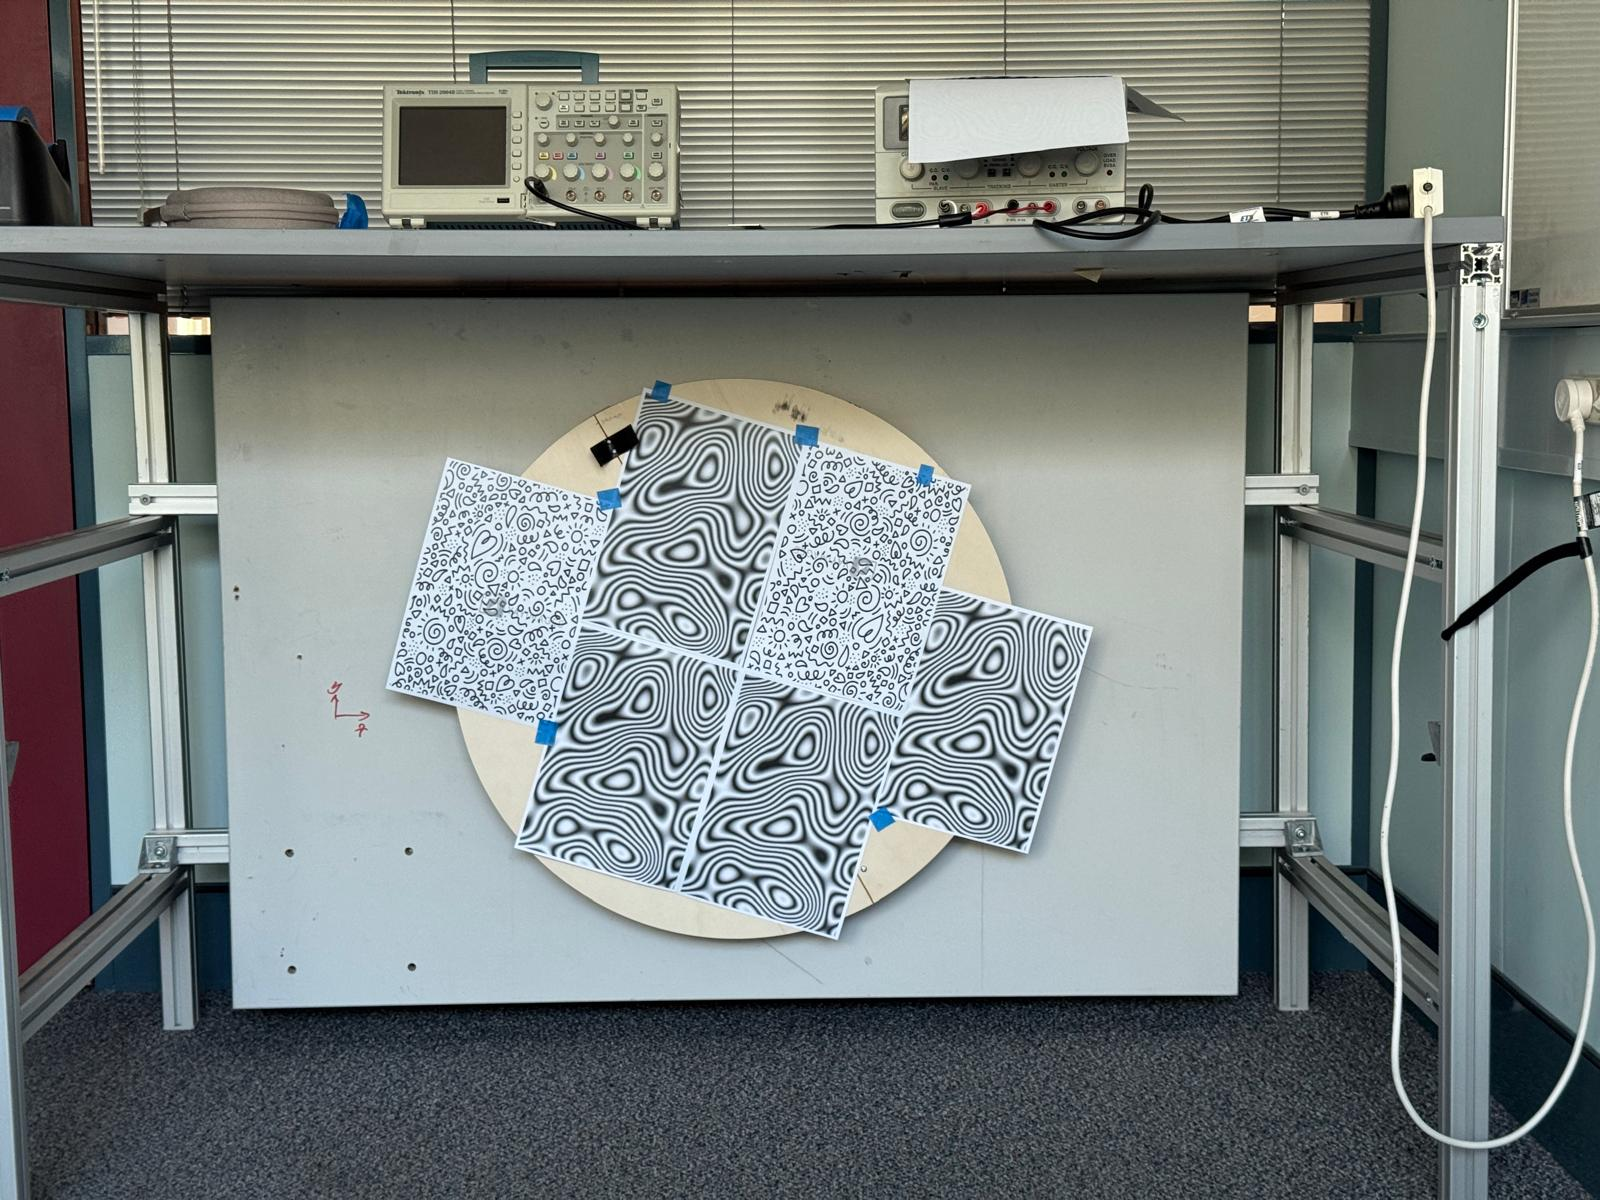
\includegraphics[width=0.85\linewidth]{images/setup_2.jpeg}
  \caption{Experimental apparatus. The event camera (tripod-mounted, off-camera right) views a patterned wooden disc mounted on a rotating spindle. The disc features six high-contrast paper patterns affixed with blue tape, creating varied edge structures for rich event generation. The grey mounting board provides a stable backdrop with a hand-drawn coordinate system (red $x$/$y$ axes, lower-left). Ambient room lighting was used.}
  \label{fig:rig}
\end{figure}

% Removed duplicate close-up image; only the first overview image remains
% \begin{figure}[t]
%   \centering
%   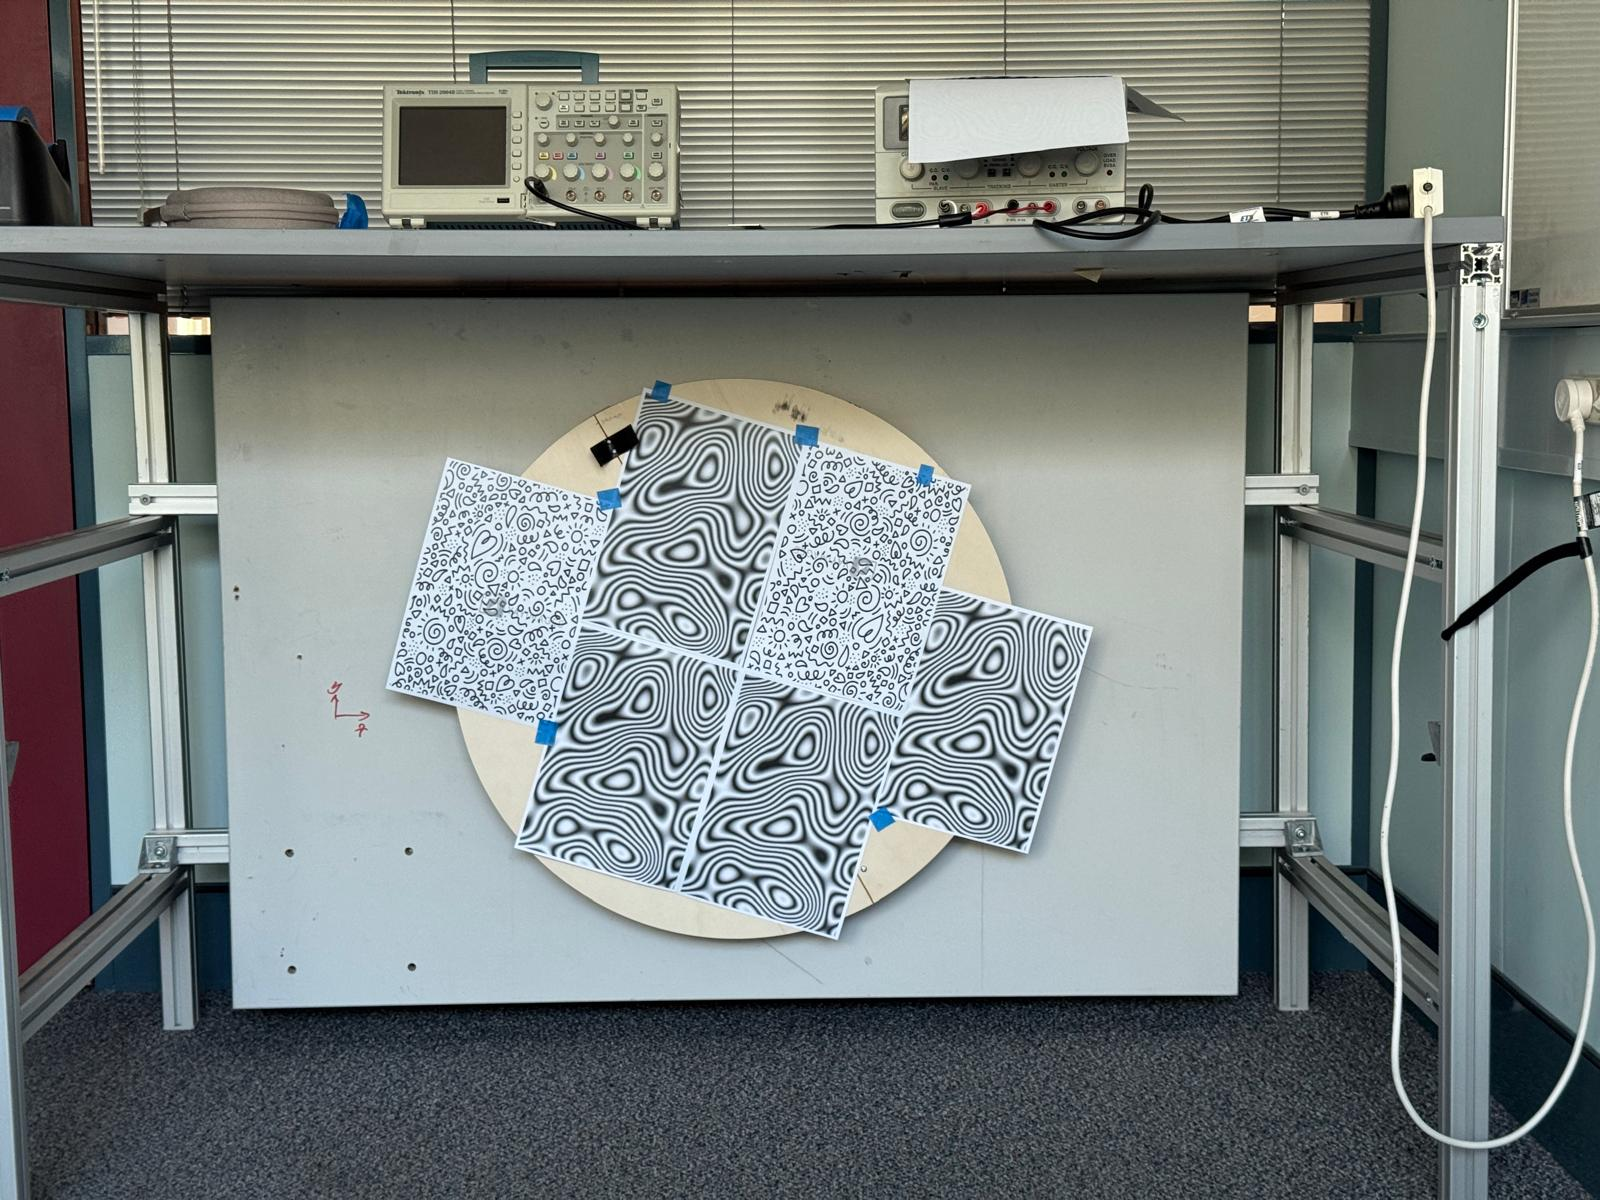
\includegraphics[width=0.7\linewidth]{images/setup_2.jpeg}
%   \caption{Close-up view of the patterned disc face. Six square paper patterns are arranged in a grid, secured with blue tape at the corners. Four patterns (center and lower rows) feature flowing concentric black and white lines creating curved edge structures. Two patterns (top corners) contain dense random assortments of shapes (squiggles, stars, circles, hearts) for high-frequency spatial content. This variety of textures ensures comprehensive testing of the cancellation algorithm under different edge orientations and densities.}
%   \label{fig:disc}
% \end{figure}

% ============================================================
\section{Datasets and Protocol}
\label{sec:datasets}

\subsection{Sequences}
We recorded multiple \emph{spinning-disc} sequences by varying the rotation rate and exposure to stress different motion regimes. Each sequence contains the raw, time-ordered event stream:
\[
E = \big\{ (x_i, y_i, p_i, t_i) \big\}_{i=1}^{N},
\]
with timestamps in microseconds (converted to seconds in software). For most analyses we also used a tracker CSV with center and angular-velocity estimates; when absent, these were inferred from events via circle fit and angle differencing (Chapter~\ref{chap:motion}).

\paragraph{Typical settings.}
We recorded sequences of 5--10\,s duration per capture, at rotation rates spanning 1.5--3.5\,rev/s ($\omega \approx 1.5--3.5$\,rad/s), to study the dependence of cancellation on angular velocity $\omega$ and radial phase speed $r|\omega|$. For the disc radius $r \approx 264$\,px imaged at this setup, the maximum circumferential velocity at the rim reached $\sim 800$\,px/s, creating high apparent motion to stress-test the temporal gating mechanism. Lighting and camera pose remained fixed across repeats within a set to ensure consistency.

\subsection{Protocols and Repeats}
All analyses were performed on one primary recording (and, where noted, one supplementary sequence). Parameter sweeps changed \emph{software} settings only (e.g., $\Delta t$, $\epsilon_{xy}$, $\epsilon_t$, polarity mode, $\omega$-bias) on the \emph{same} recordings; no repeated acquisitions were performed. Each sweep used identical temporal extents (three non-overlapping windows per sequence) to enable cross-window comparison.

\subsection{Data Splits}
No learning was employed; thus no train/validation/test split was required. Instead, we designate \emph{analysis windows} (e.g., W1, W2, W3) within each sequence and report per-window curves (cancellation vs.\ parameter) as well as their mean and standard deviation. When a tracker CSV for $(\hat c,\hat\omega)$ was available, we used it directly and interpolated to event times (Chapter~\ref{chap:motion}); otherwise $(\hat c,\hat\omega)$ were estimated from the events as described in Chapter~\ref{chap:motion}.

\subsection{Summary Table}
Table~\ref{tab:sequences} summarizes the datasets used in the study.

\vspace{0.5\baselineskip}
\begin{table}[H]
  \centering
  \small
  \caption{Sequences used in experiments. ``Rate'' is the nominal spin frequency. $N$ is total events in the sequence. Analysis windows W1--W3 are non-overlapping 10\,ms slices used for robustness checks.}
  \label{tab:sequences}
  \begin{tabularx}{\linewidth}{@{} l c c c c X @{} }
    \toprule
    \textbf{Seq.} & \textbf{Duration (s)} & \textbf{Rate (rad/s)} & \textbf{Windows} & \textbf{$N$ (events)} & \textbf{Purpose} \\
    \midrule
    Disc-PWM1280 & 10.0 & $\sim 3.6$ & W1--W6 & $\sim 36.3 \times 10^6$ & Primary analysis \\
    \bottomrule
  \end{tabularx}
\end{table}

\paragraph{Throughput note.}
For rapid iteration, we use short analysis windows (W1--W6, 10\,ms each) to obtain quick, stable estimates with low compute cost. To validate consistency over extended durations, we also analyzed representative subsets (50,000 events) from 5-second windows across a range of prediction horizons $\Delta t$, demonstrating stable CR trends and exponential decay characteristics over longer temporal extents; the corresponding fine-resolution plots are provided in Chapter~\ref{chap:results}. The 50,000-event sample size provides statistical precision of $\pm 0.08\%$ on cancellation rate estimates (95\% confidence interval), which is negligible compared to motion estimation uncertainty ($\sim 0.5$--1%) and enables computationally tractable analysis while preserving statistical validity.

\paragraph{Data characteristics.}
The dataset comprises a single continuous 10-second recording. The motor driver PWM was set to 1280\,Hz to control the spinning speed; the event camera is asynchronous and has no fixed sampling rate. The sequence contains three distinct high-contrast patterns (visible in Fig.~\ref{fig:rig}), creating varied edge densities across the disc face. Analysis was performed on six non-overlapping 10\,ms windows (W1--W6) extracted at $t=5.0,\,5.01,\,8.20,\,8.21,\,9.00,\,9.01$\,s, enabling statistics across temporal variations in motion estimation and event density.

% ============================================================
\section{Software Pipeline}
\label{sec:software}

\subsection{Overview}
Figure~\ref{fig:pipeline} outlines the causal, per-event pipeline:

\begin{enumerate}
  \item \textbf{I/O \& preprocessing:} Load events CSV/NPY; map polarities to $\{0,1\}$ or $\{\pm 1\}$; convert timestamps to seconds; time-sort (if needed).
  \item \textbf{Motion estimation:} Obtain $(\hat c(t),\hat\omega(t))$ from tracker CSV or compute from events (circle fit $\rightarrow$ angles $\rightarrow$ finite differences), then smooth and store as time series.
  \item \textbf{Event prediction:} For each event $e_i=(x_i,t_i,p_i)$, compute $x_i' = \mathcal{R}\!\big(x_i; \hat c(t_i), \hat\omega(t_i)\Delta t\big)$ and predicted time $t_i' = t_i+\Delta t$.
  \item \textbf{Temporal gating:} At the current processing time $\tau$, pop predictions with $|t_i' - \tau| \le \epsilon_t$ and gather real events $e_j$ with $|t_j - t_i'| \le \epsilon_t$.
  \item \textbf{Spatial \& polarity gating:} Accept candidates with $\|x_j - x_i'\|_2 \le \epsilon_{xy}$ and polarity predicate satisfied (default: opposite).
  \item \textbf{One-to-one pairing:} Mutual-nearest-neighbor (MNN) check within the gated sets; greedily accept pairs in ascending distance to prevent many-to-one matches.
  \item \textbf{Cancellation / anti-event:} Remove matched pairs from the stream (or emit an anti-event at $(x_i',t_i',-p_i)$ in a signed raster accumulator).
  \item \textbf{Metrics \& visualization:} Compute cancellation ratio, residual densities (disc vs.\ background), and generate high-pass videos via bilinear splatting.
\end{enumerate}

\begin{figure}[t]
  \centering
  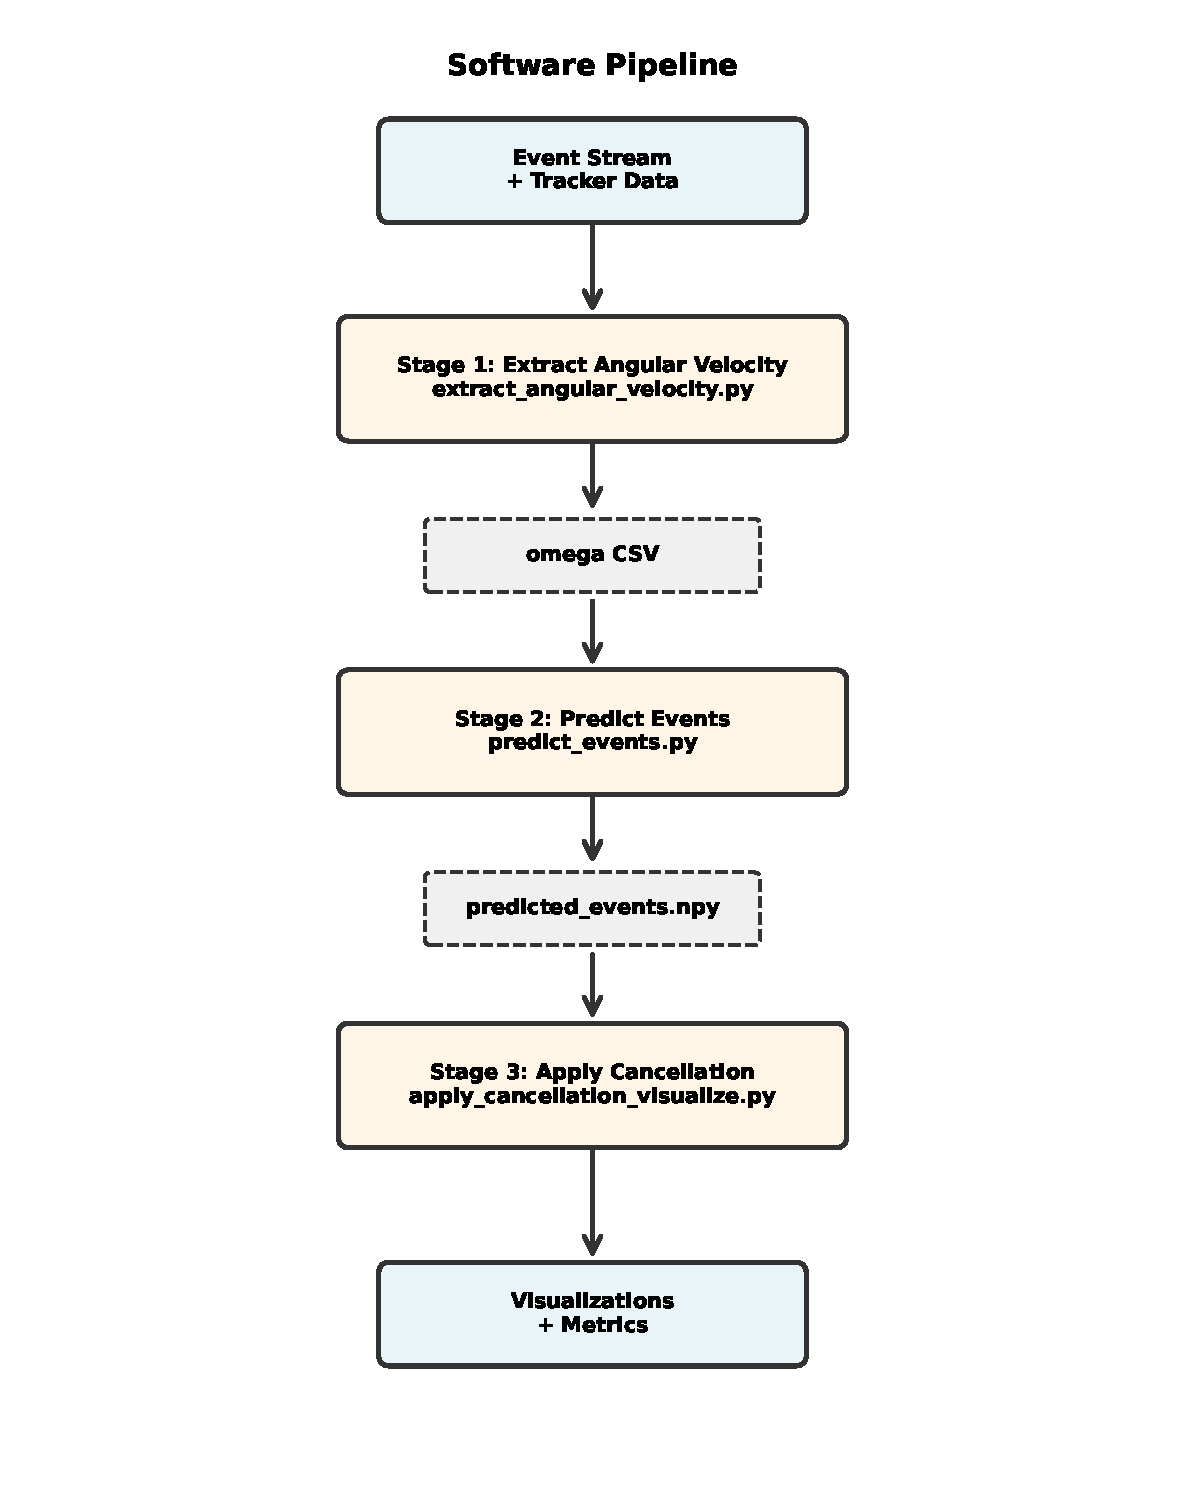
\includegraphics[width=0.55\linewidth]{figures/pipeline_flowchart.pdf}
  \caption{Software pipeline overview. The three-stage processing flow: (1) extract angular velocity from tracker data, (2) predict future event locations using the motion model, and (3) apply spatiotemporal cancellation and generate visualizations. All stages operate causally with bounded buffers.}
  \label{fig:pipeline}
\end{figure}

\subsection{Implementation Details}
We implemented the pipeline in Python:
\begin{itemize}
    \item \textbf{Environment:} Python~3.8+, NumPy (1.21+), SciPy (cKDTree for spatial indexing), pandas (data analysis), matplotlib/seaborn (visualization), opencv-python (optional: additional image processing).
  \item \textbf{Precision:} Coordinates and polarity as \texttt{float32}; timestamps as \texttt{float64}. Trigonometric rotation uses radians.
  \item \textbf{Interpolation:} Linear \texttt{interp1} for $\hat c(t)$, $\hat\omega(t)$ at \emph{event times} $t_i$ with edge-hold.
  \item \textbf{Temporal buffers:} A min-heap keyed by $t'$ for predictions; a deque for recent real events; two indices maintain the $[t'-\epsilon_t,\,t'+\epsilon_t]$ window.
  \item \textbf{Spatial index:} KD-tree (SciPy) or uniform grid on gated candidates. Matching performed with MNN to enforce one-to-one.
  \item \textbf{Rasterization:} Signed bilinear splatting of residual (uncancelled) events for stable visualization; optional nearest-neighbor for ablation.
  \item \textbf{Parameters (defaults):} $\Delta t \in [0.25, 2]$\,ms, $\epsilon_t \in [0.25, 1.0]$\,ms, $\epsilon_{xy}\in [1.5, 3.0]$\,px; polarity mode = \texttt{opposite}.
\end{itemize}

\subsection{Runtime and Throughput}
On the workstation used (AMD Ryzen 9 5900HX, 8 cores/16 threads; 32\,GB RAM), processing proceeds in small buffered chunks of events to balance memory usage and efficiency while preserving per-event causality. Inner loops use NumPy for speed, but all matching decisions remain per-event at their decision times; the dominant cost is spatial neighborhood querying within the temporal gate. Typical throughputs observed:

\begin{itemize}
  \item \textbf{Prediction:} $\geq 50$ million events/s (pure vectorized rotation with NumPy), limited only by memory bandwidth.
  \item \textbf{Matching (with $N=30,000$ events per temporal slice):} $\sim 5--10$ thousand matched pairs/s (cKDTree construction + nearest-neighbor queries). The bottleneck is the spatial indexing for each event, which scales as $O(N \log N)$.
  \item \textbf{Full pipeline (per $10^6$ events):} $\sim 10--20$ seconds end-to-end (I/O, estimation, prediction, matching, metrics), enabling interactive parameter sweeps on modest hardware.
  \item \textbf{Visualization:} Real-time generation of PNG frames with signed-bilinear splatting; MP4 encoding (if performed) is bounded by I/O rather than compute.
\end{itemize}

For the comprehensive parameter sweep (DT values 0--20\,ms, 5 spatial tolerances, 5 temporal tolerances = 525 combinations), total processing time on a single workstation ranged from $4--8$ hours depending on dataset size ($\sim 30$\,M events), demonstrating the feasibility of thorough sensitivity analysis.

\subsection{Reproducibility and Configuration}
All experiments are driven by a single configuration file specifying $(\Delta t,\epsilon_t,\epsilon_{xy})$, polarity mode, interpolation method, and output paths. Randomness is not used beyond the optional RANSAC in circle fitting (seed fixed). Each run stores a manifest containing code commit ID, parameter values, and checksums for input files.

\subsection{Safety Checks and Diagnostics}
We embed invariants to guard against silent errors:
\begin{itemize}
  \item Each real/predicted index can appear in at most one match.
  \item Predictions leaving the image are dropped before indexing.
  \item With exact parameters and $\Delta t\to 0$, cancellation $\to 100\%$ on synthetic rings.
  \item The measured CR vs.\ $\Delta t$ decays smoothly (no bin-edge artifacts), confirming the \emph{true temporal gate}.
  \item Residual radial profiles flag center bias: a uniform offset indicates $\|\Delta c\|$; widening with radius indicates $\Delta\omega$ drift.
\end{itemize}

\medskip
\noindent\textbf{Summary.} The apparatus isolates rotational ego-motion with a reproducible, high-contrast target, while the software stack enforces strictly causal, per-event processing. This combination allows controlled sensitivity studies over $\Delta t$, spatial/temporal tolerances, polarity handling, and model biases, which we report in Chapter~\ref{chap:metrics}.
